\documentclass[a4paper,11pt]{article} 

\usepackage[T1]{fontenc}
\usepackage[utf8]{inputenc}

\usepackage{multirow} 
\usepackage{booktabs} 
\usepackage{graphicx} 
\usepackage{setspace}
\usepackage[skip=6pt plus1pt, indent=0pt]{parskip}

\usepackage{float}
\usepackage{fancyhdr}

\usepackage{tcolorbox}
\usepackage{hyperref}
\hypersetup{
    colorlinks=true,
    linkcolor=blue,
    filecolor=magenta,      
    urlcolor=blue
}

\usepackage[margin=1in]{geometry}
\usepackage{enumitem}
\newlist{steps}{enumerate}{1}
\setlist[steps, 1]{label = Step \arabic*:}
\newcommand{\incode}[1]{
\begin{tcolorbox}[colback=blue!5!white, boxrule=0mm, sharp corners]
\texttt{#1}
\end{tcolorbox}
}

\newcommand{\note}[1]{\textit{\textcolor{gray}{#1}}}

\pagestyle{fancy} 
\fancyhf{} 
\lhead{Advanced Computer Networks 2022}
\rhead{Lin Wang, George Karlos, Florian Gerlinghoff} 
\cfoot{\thepage} 

\begin{document}


\thispagestyle{empty} 

\begin{tabular}{@{}p{15.5cm}} 
{\bf Advanced Computer Networks 2022} \\
Vrije Universiteit Amsterdam \\
Lin Wang, George Karlos, Florian Gerlinghoff \\
\hline 
\\
\end{tabular} 

\vspace*{0.3cm} 

{\Large \bf Lab5: Switches Do Dream Of Machine Learning! (Report)} 

\vspace*{0.3cm} 

%============== Please do not change anything above ==============%

% Please modify this part with your group information
\begin{tcolorbox}[sharp corners, colback=blue!5!white]
\begin{tabular}{@{}ll}
\textbf{Group number:} & 9 \\
\textbf{Group members:} & Hsiang-ling Tai, Yung-sheng Tu, Sicheng Peng \\
\textbf{Slip days used:} & 3 \\
\textbf{Bonus claims:} & Nee \\
\end{tabular}
\end{tcolorbox}

\vspace{0.4cm}

\section{Basic In-Network Aggregation}
\subsection{Overview}
\begin{itemize}
    \item \textbf{What do workers do?} \\
    The goal of every worker is to send a \textbf{\textit{vector}} containing \textit{\textbf{N elements}} (32-bit integer) to the switch and receive the sum of all workers' vectors from the switch. Each worker would only send \textit{\textbf{CHUNK\_SIZE elements}} per packet to switch. Therefore, \({N}/{CHUNK\_SIZE}\) packets are required to send all the elements in the vector to the switch. After sending a packet, workers would receive a packet containing \textit{\textbf{CHUNK\_SIZE elements}}, which is the sum of all workers' chunks, and then proceeds to send the next chunk of data.
    \item \textbf{What does the switch do?} \\
    The goal of the switch is to aggregate \textit{\textbf{CHUNK\_SIZE elements}} which constitute each packet from all workers. After receiving all packets of the same chunks from all workers, the switch would broadcast the packet containing \textit{CHUNK\_SIZE} aggregate elements to all the workers, and then continue waiting for the next chunk of data.
    \item \textbf{Scenario} \\
    Assuming that only \textit{worker0} and \textit{worker1} are connected to the switch, \textit{CHUNK\_SIZE} is 32, and there are 2048 elements in a \textit{vector}. Both \textit{worker0} and \textit{worker1} would send a packet containing the first 32 elements of the vector. After receiving these two packets, the switch would aggregate their elements and then broadcast the packet with 32 aggregate elements back to \textit{worker0} and \textit{worker1}. Workers would continue doing this until they have sent and received 64 packets \textit{(2048 elements/CHUNK\_SIZE 32)} from the switch.
\end{itemize}


\subsection{Communication}
\label{sec:communicate}
\begin{figure}[htbp]
    \centering
    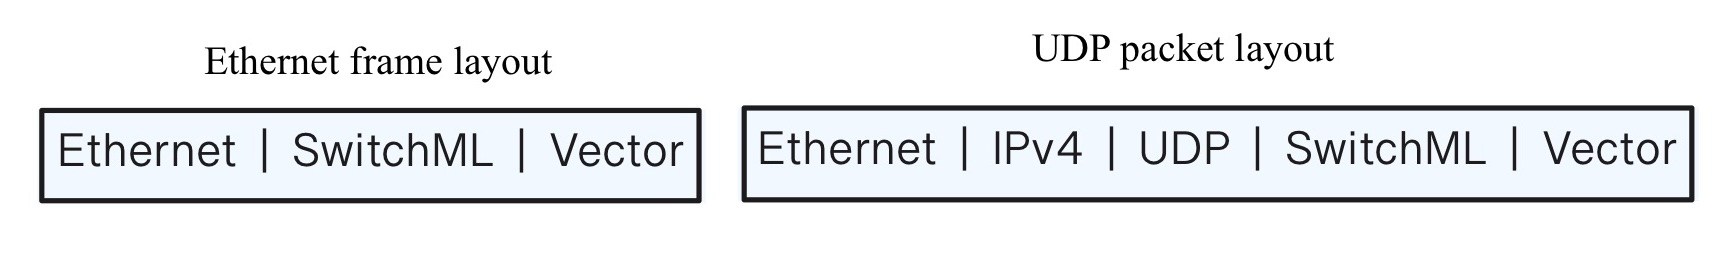
\includegraphics[width=14cm]{header_layout.jpg}
    \caption{Ethernet frame and UDP packet}
    \label{fig:hdr}
\end{figure}

Both the Ethernet frame and UDP packet contain SwitchML header and Vector header (see Figure \ref{fig:hdr}). The \textbf{SwitchML header} is made up of \textbf{rank} and \textbf{num\_workers} fields. The \textbf{\textit{rank}} field indicates the worker sent the packet, and the \textit{\textbf{num\_workers}} field shows the number of workers. These two fields allow the switch to track whether all workers have sent the packet. The \textbf{Vector header} consists of \textit{CHUNK\_SIZE} elements, all of which are 32-bit integers, which is the target data we are going to aggregate.
\begin{itemize}
    \item \textbf{Ethernet Communication} (level 1) \\
    \label{level1comm}
    Workers use Scapy to craft, send and receive Ethernet frames. The \textbf{EtherType is set to 0x8787} when workers send an Ethernet frame which contains a SwitchML header and Vector header as payload to the switch. Hence, when the switch parses the Ethernet header and finds that the EtherType is 0x8787, it would continue to parse the SwitchML header and Vector header. In addition, \textbf{0x8787} has not been used by some notable protocols, so we consider it as a good number. 
    \item \textbf{UDP Communication} (level 2) \\
    \label{udpcmn}
    
    \begin{figure}[htbp]
        \centering
        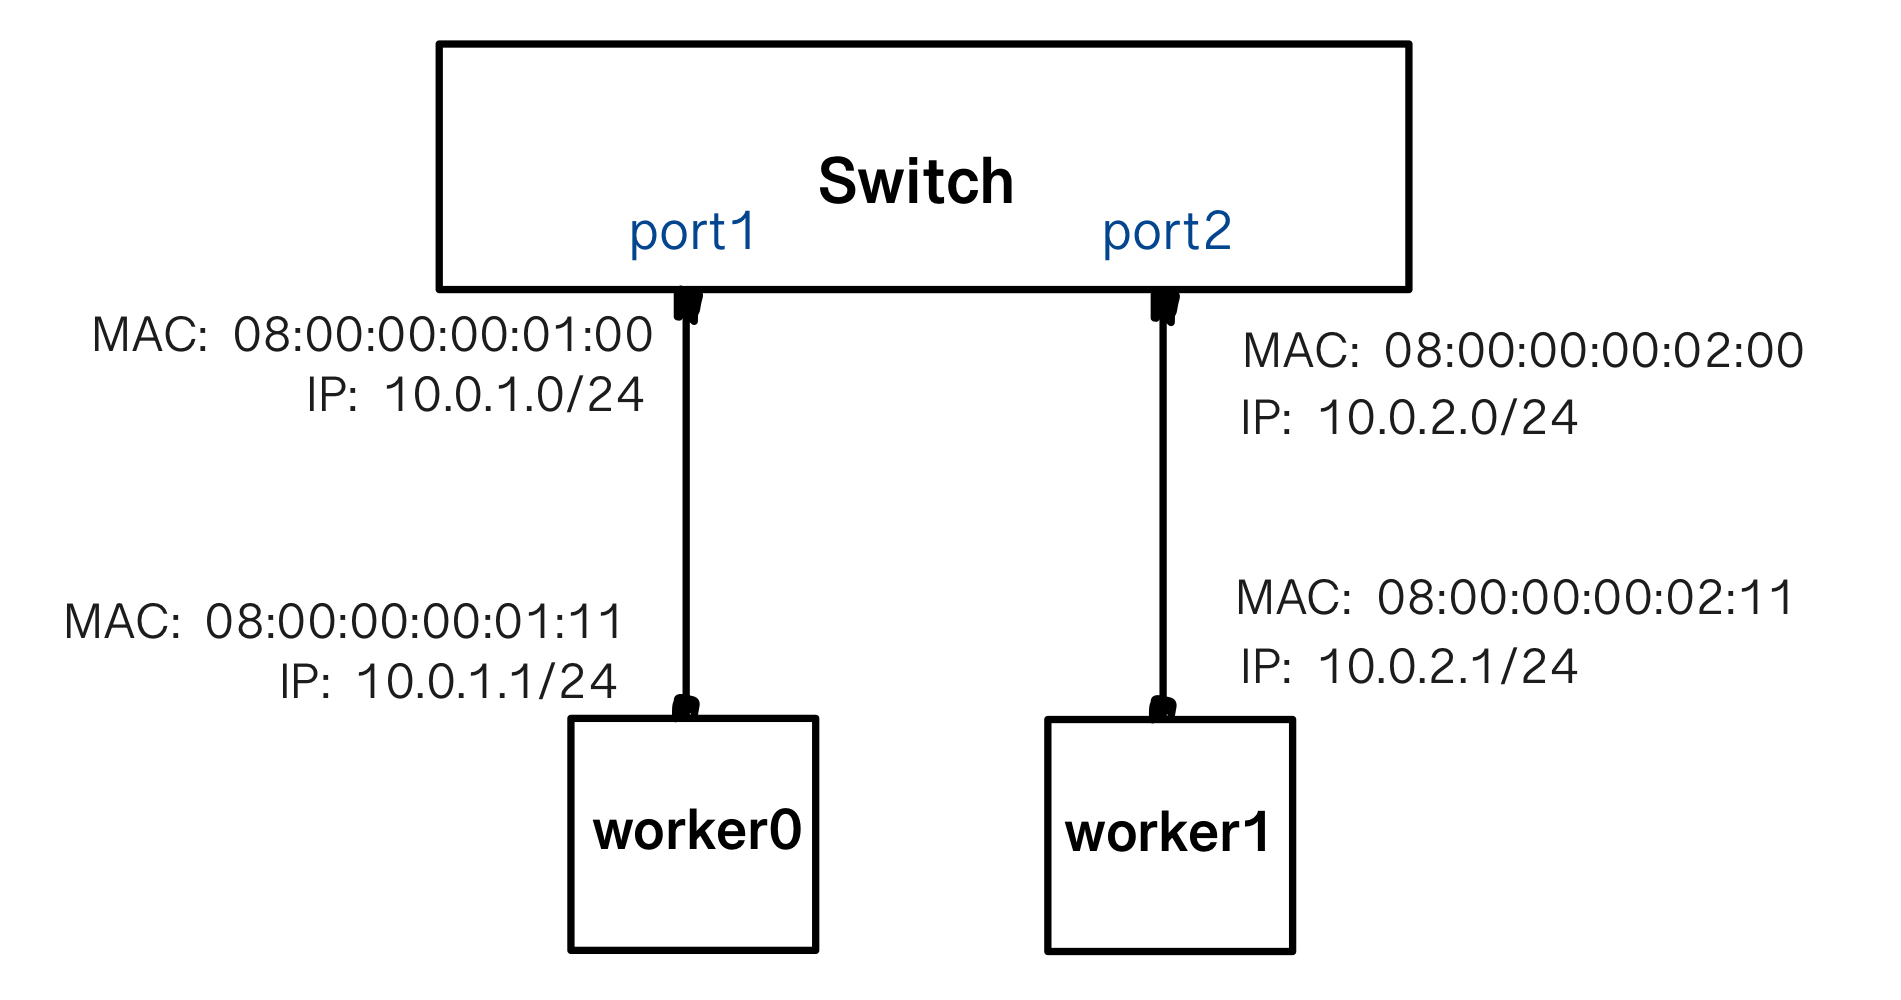
\includegraphics[width=10cm]{udp_switch.jpeg}
        \caption{The topology of switch and workers}
        \label{fig:udpsw}
    \end{figure}
    
    The \textbf{destination port in UDP header} is set to \textbf{38787} when workers send SwitchML packets to the switch through a socket. So when the switch parses the UDP header and finds that the destination port is 38787, it would continue to parse the SwitchML header and Vector header. However, before sending the first UDP packet, every worker would send an ARP request to the switch for the MAC Address of the interface to which it is linked. In order to send an ARP reply from the switch, \textit{\textbf{num\_workers}} (1 to 8) entries would be added to \textbf{\textit{tbl\_arp}} table during the one-time control plane configuration. The key of \textit{tbl\_table} is the ingress port and the action is arp\_reply which generates an ARP reply. All required fields of an ARP reply can be retrieved from the corresponding ARP request except the \textbf{source MAC address} (the MAC address of the switch). Therefore, the source MAC address will be the parameter of the arp\_reply action. For example, as shown in Figure \ref{fig:udpsw}, worker0 is connected to switch port1, and worker1 is connected to port2. It will have two entries set up by the one-time control plane. The key of the first entry is \textbf{1} (port1) and the action is arp\_reply with parameter \textbf{08:00:00:00:00:01:00} (the MAC Address of the switch port1); the key of the second entry is \textbf{2} (port2) and the action is arp\_reply with parameter \textbf{08:00:00:00:00:02:00} (the MAC Address of the switch port2).
    %\textbf{worker: \\}
    %First, set up a UDP socket, and bind workers' IP addresses which we obtained from \textit{\textbf{ip()}} and our preferred port (\textbf{38787}) to it. \\
    %Then, before workers send a SwitchML packet to the switch, it has to know the switch's IP address and MAC address. We acquired the switch's IP address from the network configuration Scapy got, and its Mac address would get automatically when sending packets through the UDP socket, i.e. the socket would send an ARP packet at first and send UDP packets with the known switch's Mac address. \\
    %Lastly, generate SwitchML packets as UDP packets' payload to send to the switch and update the result per chunk after receiving the aggregated result.
\end{itemize}


\section{Basic Implementation}
\subsection{Configuration}
Several configurations should be determined beforehand, including \textit{CHUNK\_SIZE} and \textit{multicast group}.\\
\begin{itemize}
    \item CHUNK\_SIZE \\
    \label{chunksize}
    Our \textbf{CHUNK\_SIZE is 32}. The larger \textit{CHUNK\_SIZE} is, the fewer packets workers send per iteration. Therefore, we would like to find out the maximum of \textit{CHUNK\_SIZE}. One of the \textit{Requirements and Assumptions} of this assignment says, ‘A single switch pipeline can perform at most 32 aggregations per packet traversal’, which means it could only have a maximum of 32 aggregation stages. Furthermore, the register could only read/write once per stage, which indicates that only 1 element could be aggregated per stage. As a result, \textit{CHUNK\_SIZE} is at most 32.
    \item Multicast Group \\
    The multicast group is added by the one-time control plane in \textit{network.py}. The multicast group ID is 1 and the ports are all the ports connected to workers. Thus, when the multicast group ID is set to 1, all workers would receive the packet from the switch.
\end{itemize}
% \subsection{SwitchML header and Vector header}
\subsection{Aggregation}
The aggregation method is the same no matter whether packets are sent over Ethernet or UDP.

\begin{figure}[htbp]
    \centering
    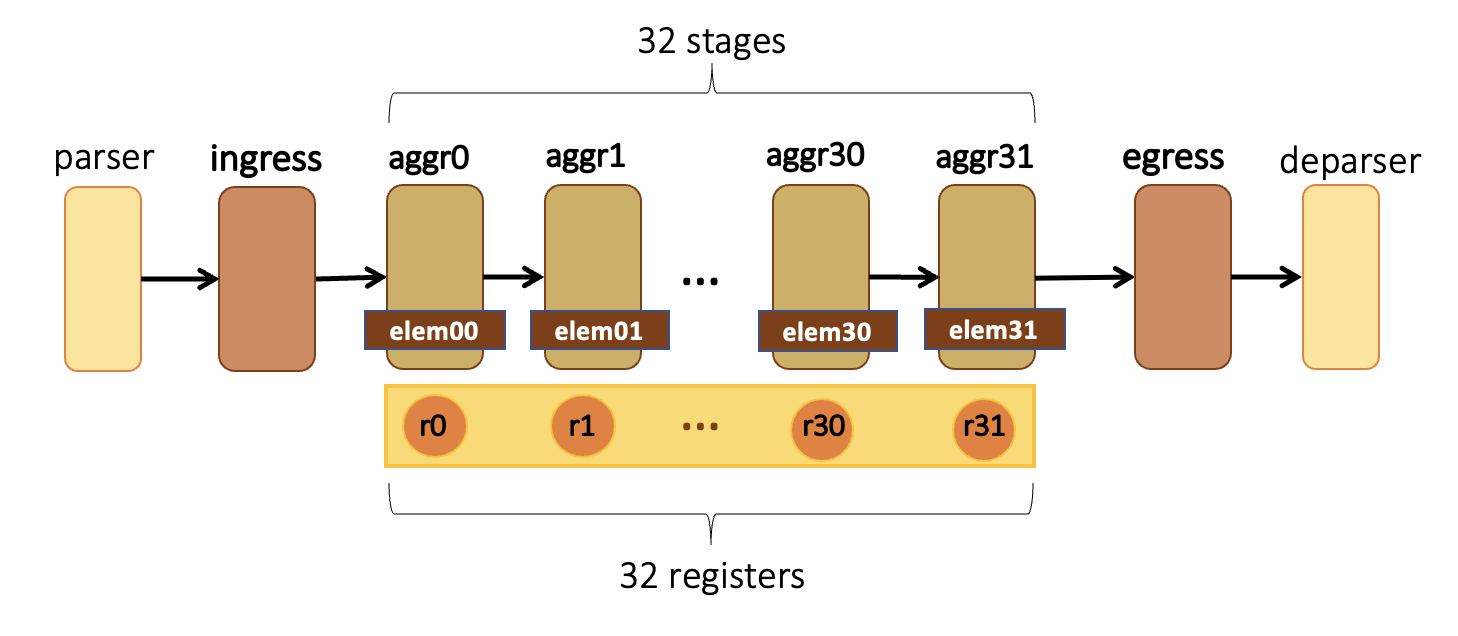
\includegraphics[width=13cm]{dataflow.png}
    \caption{\textbf{elem00 to elem31} is a chunk of data in each packet, and \textbf{r0 to r31} is a register which belongs to stage \textbf{aggr0 to aggr31}}
    \label{fig:df}
\end{figure}

\begin{itemize}
    \item \textbf{Ingress Stage} \\
    \label{ingstg}
    In the \textit{ingress stage}, it would maintain an 8-bit register (the number of workers is 1 to 8) to record the arrival of workers based on their \textit{rank}. The value of the register would be stored in \textit{\textbf{meta.all\_worker\_arrived}} and then passed to the \textit{aggregation stage}. Note that this register would be reset to 0 for the next chunk of data when the last worker arrived.
    \item \textbf{Aggregation Stage} \\
    \label{aggstg}
    As shown in Figure \ref{fig:df}, the switch would have 32 identical aggregation stages with the default actions \textbf{\textit{aggr()}}. Stage \textit{aggr0} would aggregate \textit{elem00} from all workers, stage \textit{aggr1} would aggregate \textit{elem01} from all workers, and so on. For example, when the first stage \textit{\textbf{aggr0}} receives \textit{\textbf{elem00}} as input, the action \textbf{\textit{aggr()}} would do:
    \begin{steps}[leftmargin=2cm, label=\textbf{Step \arabic*}:]
        \item Read the value in register \textit{\textbf{r0}}, the sum of elem00s of other arrived workers.
        \label{aggstep1}
        \item Aggregate the value of r0 with \textbf{\textit{elem00}} as \textit{elem\_tmp}.
        \item Update the result \textit{elem\_tmp} back to register \textbf{\textit{r0}}.
        \item Increase \textit{\textbf{meta.elem\_idx}}.
        \item Go to the next stage \textbf{\textit{aggr1}}.
        \label{aggstep5}
    \end{steps}
    In \textit{Step 5}, \textbf{\textit{meta.elem\_idx}} is the counter in metadata and is used as the register index. It starts from 0 and adds 1 before going to the next stage. For example, at stage \textit{aggr0}, \textit{meta.elem\_idx} is 0, so \textit{aggr()} would access \textit{r0}; at stage \textit{aggr1}, \textit{meta.elem\_idx} is 1, so aggr() would access \textit{r1}, and so forth. \\
    Normally, \textit{aggr()} does above \textit{Step1 to Step5} to deal with all packets. But it would be slightly different \textbf{when the packet is sent by the last worker}, which could be revealed by \textbf{\textit{meta.all\_worker\_arrived}} as the \hyperref[ingstg]{Ingress Stage} mentioned. For example, when the first stage \textit{\textbf{aggr0}} receives \textit{\textbf{elem00}} as input, the action \textbf{\textit{aggr()}} would do:
    \begin{steps}[leftmargin=2cm, label=\textbf{Step \arabic*}:]
        \item Read the value in register \textit{\textbf{r0}}, the sum of elem00s of other arrived workers.
        \label{aggstepl1}
        \item Aggregate the value of r0 with \textbf{\textit{elem00}} as \textit{elem\_tmp}.
        \item Reset the register \textit{r0} to \textbf{0}.
        \label{aggstepl3}
        \item Update the result \textit{elem\_tmp} to \textit{\textbf{elem00}} in packet's header.
        \item Increase \textit{\textbf{meta.elem\_idx}}.
        \item Set up multicast group which would broadcast to every worker.
        \item Go to the next stage \textbf{\textit{aggr1}}.
        \label{aggstepl7}
    \end{steps}
    To clarify, the difference in \textit{Steps 3}, \textit{4}, and \textit{6} is because the arrival of the last worker indicates the aggregation is done in this chunk. So the register should be reset for the next chunk of data, and the result would be written in the header and then broadcast to every worker.
    \item \textbf{Egress Stage} \\
    If it is sent over Ethernet, nothing would be done; however, if sent over UDP, the IP address and MAC address would be updated (see Section \hyperref[sec:Broadcast]{2.3}).
\end{itemize}
\subsection{Broadcast the Result}
\label{sec:Broadcast}
\begin{itemize}
    \item \textbf{Ethernet} (level 1) \\
    For Ethernet, packets would be multicast to every worker after the multicast group is set as mentioned earlier.
    \item \textbf{UDP} (level 2) \\
    \label{broadcastudp}
    For UDP, besides setting the multicast group as level 1, the source and destination of both the IP address and MAC address have to be updated before sending. In addition, the checksums of IPv4 and UDP should be updated as well. To update the IP address and MAC address, \textit{\textbf{num\_workers}} (1 to 8) entries would be added in the \textbf{\textit{tbl\_sml\_udp}} table during the one-time control plane configuration. The key of \textit{tbl\_sml\_udp} is the egress port and the action is to update data with parameters, including IPv4 address, destination IP address, source MAC address and destination MAC address. For example, as shown in Figure \ref{fig:udpsw}, worker0 is connected to switch port1 and worker1 is connected to port2. It will have two entries set up by the one-time control plane. The key of the first entry is \textbf{1} (port1), and the action is to update the source IP address to \textbf{10.0.1.0}, destination IP address to \textbf{10.0.1.1}, source MAC address to \textbf{08:00:00:00:01:00} and destination MAC address to \textbf{08:00:00:00:01:11}. Note that these four addresses are passed as action parameters in the one-time control plane configuration.
\end{itemize}

\newpage
\section{Fault-Tolerant Aggregation Protocol}
\label{ftap}
\label{sec:ftap}
The method of communication is no different from \hyperref[udpcmn]{UDP Communication}. The only difference is that we add a new field, \textbf{\textit{chunk\_id}}, in the SwitchML header. In the fault-tolerant scenario, workers would re-transmit the packet when timeout, so it would have different chunks of data, some belonging to the previous aggregation stage and others belonging to the current one, reaching the switch. The \textit{chunk\_id} can help the switch identify the packet as the ${n}^{th}$ chunk of data. The \textit{chunk\_id} would be either \textbf{0} (\textit{n} is even) or \textbf{1} (\textit{n} is odd). First of all, a worker would only send the ${n}^{th}$ chunk when it has received the ${n-1}^{th}$ chunk, but some other workers might stuck in the ${n-1}^{th}$ one due to failures. This means that the ${n}^{th}$ chunk would also get stuck because it has not received the data from workers stuck in the ${n-1}^{th}$ chunk yet. That is to say, to accomplish fault tolerance over UDP, the switch would only encounter 2 different chunks of data (${n-1}^{th}$ and ${n}^{th}$). The ${n-1}^{th}$ chunk would be kept in registers until all workers move on to the ${n}^{th}$ chunk for fault tolerance.


\section{Fault-Tolerant Implementation}
\label{sec:fti}
As \hyperref[sec:ftap]{section 3} mentioned, the switch has to store the previous chunk for fault tolerance. Therefore, the register in the \hyperref[ingstg]{Ingress Stage} for recording the arrival of workers has to be 16-bit (the original is 8-bit for workers 1-8). And the 32 32-bit registers for storing the aggregation of elements in the \hyperref[aggstg]{Aggregation Stage} would be 64 32-bit registers. When \textit{chunk\_id} is \textbf{0} it would use bits \textbf{0 to 7} to store the arrival of workers and registers \textbf{0 to 31} to store elements; when \textit{chunk\_id} is \textbf{1} it would use bits \textbf{8 to 15} to store the arrival of workers and registers \textbf{32 to 63} to store elements. \\\\
When the packet come to the switch, it can be divided into the below cases (in the view of the switch):
\begin{itemize}
    \item \textbf{The packet from the worker has already been received (Re-transmit case)}
    \begin{itemize}
        \item All the workers of this chunk have already arrived \\
        This indicates the receive failure on workers or transmit failure on the switch. It should broadcast the aggregate packet to workers when all workers have arrived at the switch. In this case, the switch would go through 32 aggregation stages to read the value from the registers (just like \hyperref[aggstep1]{Step 1}) based on its \textit{chunk\_id} and write it to the packet header and then unicast to the port it came from.
        \item Some workers of this chunk have not arrived yet \\
        This indicates the current chunk is still doing aggregation and there are some workers who have not contributed their chunk to the switch yet. For the switch, drop this packet as it has already been aggregated. For the worker, keep waiting for the aggregated result from the switch.
    \end{itemize}
    \item \textbf{The packet from the worker is newly received (Normal case)}
    \begin{itemize}
        \item All other workers of this chunk have already arrived \\
        This is the normal case that can basically follow the \hyperref[aggstepl1]{Steps 1} to \hyperref[aggstepl7]{7} in the \hyperref[aggstg]{Aggregation Stage}. However, the switch would not do \hyperref[aggstepl1]{Step 3} which is to clear the register in that the data has to be kept for fault tolerance.
        \item The first arrived worker of this chunk \\
        This is the normal case that can basically follow the \hyperref[aggstep1]{Steps 1} to \hyperref[aggstep5]{5} in the \hyperref[aggstg]{Aggregation Stage}. Note that the register will not be reset, so the first arrived worker should overwrite the register with its current value directly instead of aggregating with the old value from the register and then updating it.
    \end{itemize}
\end{itemize}

\newpage
\section{Questions and Answers}
\begin{itemize}
    \item \textbf{Level 1} \\
    \textbf{Q: Where does a worker actually send packets to? \\}
    A: A worker sends packets to the port which connected to the switch (see details in \hyperref[level1comm]{Ethernet Communication}). \\\\
    \textbf{Q: How do hosts and the switch distinguish your protocol over other Ethernet frames?} \\
    A: The Ethertype field in the Ethernet header we set 0x8787 depicts that this Ethernet frame is used for SwitchML (see details in \hyperref[level1comm]{Ethernet Communication}). \\\\
    \textbf{Q: How many states should the switch and workers maintain and/or share?} \\
    A: Workers do not maintain any states. The switch has to maintain the arrival of workers in the register to track whether the aggregation is complete and note that this register would be reset to 0 when all workers have arrived (see details in \hyperref[ingstg]{Ingress Stage}). Also, the switch maintain the sum of chunk in the registers in \hyperref[aggstg]{Aggregation Stage}.\\\\
    \textbf{Q: What should be the value of CHUNK\_SIZE and how many values should a packet contain? \\}
    A: The value of CHUNK\_SIZE is 32. It should be as large as possible because the number of packets per iteration will decrease if the value of CHUNK\_SIZE grows (see details in \hyperref[chunksize]{Configuration} section). The header layout can find in \hyperref[sec:communicate]{Communicate}. In brief, the SwitchML header contains the \textit{rank} and \textit{num\_workers} field, and the Vector header contains 32 elements.\\\\
    \textbf{Q: How to allocate stateful memory to store intermediate aggregations on the switch? \\}
    A: There are 32 registers in the aggregation stage. The packet would go through those stages and the corresponding register would be read, aggregated with an element and then update (see details in \hyperref[aggstg]{Aggregation Stage}). \\\\
    \textbf{Q: How to (correctly) update and reuse stateful memory? \\}
    A: When the last worker chunk comes, instead of updating the sum of elements to register, it would reset the register to zero (see details in \hyperref[aggstepl3]{Step3} in Aggregation Stage). \\
    \item \textbf{Level 2} \\
    \textbf{Q: How do hosts and the switch distinguish packets in your protocol over other IP packets? \\}
    A: The destination port field in the UDP header we set 38787 depicts that this UDP packet is used for SwitchML (see details in \hyperref[udpcmn]{UDP Commnication}). \\\\
    \textbf{Q: Should the switch know the workers' IP addresses? And if so how? \\}
    A: Yes, the switch should know workers' IP addresses in that when the result packet send back to a worker, it should contain the worker's IP address and MAC address (see details in \hyperref[broadcastudp]{UDP} of section \hyperref[sec:Broadcast]{Broadcast the Result}). Otherwise, the worker would not accept the packet. 
    \\\\
    \textbf{Q: How to make sure a broadcast is correctly received by all workers' sockets? \\}
    A: The assignment description mentioned ‘Every packet sent, by both the workers and the switch, is guaranteed to be received intact’. Therefore, the switch does not care whether workers have received it or not after it broadcast the result. However, if there is the worker loses the packet in the ${n-1}^{th}$ chunk, other workers would be stuck in the ${n}^{th}$ chunk forever in that the aggregation would not be complete due to the absence of the ${n}^{th}$ chunk from that worker.\\
    % The switch does not know whether all workers' sockets have received the aggregate result, so it would maintain the previous aggregate result until the current aggregation is done. If a worker does not receive the previous result, the switch will re-transmit it to the worker. \\\\
    \item \textbf{Level 3 \\}
    \textbf{Q: What does it mean for a packet to be corrupted, and how do you recognize this? \\}
    A: If the packet UDP checksum is incorrect means the packet is corrupted. We use \textit{verify\_checksum} to verify packets' checksum and the result would be stored in \\
    \textit{standard\_metadata.checksum\_error}. If it is marked error, the packet would be dropped in the Ingress stage.
    \\\\
    \textbf{Q: How should the protocol be adapted for reliability and how much extra state (on both the switch and the workers) is required? \\}
    A: The switch has to double the registers for storing worker arrival information and for storing previous chunk elements (see detail in section \hyperref[sec:fti]{Fault-Tolerant Implementation}).
    \\\\
    \textbf{Q: How to update the switch state following the single-access memory semantics discussed in the Requirements and Assumptions of this assignment? \\}
    A: The \textit{chunk\_id} (see section \hyperref[ftap]{Fault-Tolerant Aggregation Protocol}) would help the switch to know which register it should update during the Ingress Stage (register for storing worker arrival) and Aggregation Stage (register for storing the sum of elements from every workers' chunk).
    \\
\end{itemize}


\section{References}
\begin{itemize}
    \item \href{https://buildmedia.readthedocs.org/media/pdf/scapy/latest/scapy.pdf}{Scapy Documentation}
    \item
    \href{https://www.iana.org/assignments/arp-parameters/arp-parameters.xhtml#arp-parameters-3}{ARP Parameters}
    \item
    \href{https://en.wikipedia.org/wiki/EtherType}{EtherType Wikipedia}
    \item \href{https://github.com/p4lang/p4app-switchML}{SwitchML GitHub}
    \item \href{https://p4.org/p4-spec/docs/P4-16-v1.0.0-spec.html#sec-expr-hs}{P4 docs}
\end{itemize}

\end{document}
